\documentclass[10pt]{article}

\usepackage[a4paper,margin=0.65in]{geometry}
\usepackage{amsmath,amssymb}
\usepackage{graphicx}
\usepackage{booktabs}
\usepackage{array}
\usepackage{float}
\usepackage{hyperref}
\usepackage{enumitem}
\usepackage{xcolor}
\usepackage{tikz}
\usetikzlibrary{positioning,arrows.meta,shapes.geometric,fit,calc}

\setlist{nosep,leftmargin=*}
\renewcommand{\arraystretch}{1.2}
\setlength{\parindent}{0pt}
\setlength{\parskip}{2pt}

\tikzset{
layer/.style={
draw,
rounded corners,
minimum width=1.7cm,
minimum height=0.65cm,
align=center,
fill=blue!10,
font=\scriptsize
},
smalllayer/.style={
draw,
rounded corners,
minimum width=1.35cm,
minimum height=0.58cm,
align=center,
fill=green!10,
font=\scriptsize
},
arrow/.style={
-{Latex[length=2mm]},
thin
}
}

\newcommand{\figblock}[3]{%
\begin{figure}[H]
\centering
\includegraphics[width=#2\textwidth]{figures/#1}
\caption{#3}
\end{figure}
}

\begin{document}

%%%%%%%%%%%%%%%%%%%%%%%%%%%%%%%%%%%%%%%%%%%%%%%%%%%%%%%%%%%%
% TITLE
%%%%%%%%%%%%%%%%%%%%%%%%%%%%%%%%%%%%%%%%%%%%%%%%%%%%%%%%%%%%

\begin{center}

{\large\textbf{Shiv Nadar University Chennai}}

\vspace{2mm}

{\normalsize\textbf{CS3807 -- Deep Learning Laboratory}}

\vspace{2mm}

{\large\textbf{Experiment 6}}

\vspace{1mm}

{\normalsize\textbf{End-to-End Study of RNN, LSTM and GRU for}}

{\normalsize\textbf{Sequence Learning and Video Understanding}}

\end{center}

\vspace{3mm}

\begin{tabular}{|p{3.4cm}|p{9.0cm}|p{1.4cm}|}
\hline
Degree \& Branch &
B.Tech Artificial Intelligence \& Data Science &
Semester V\\
\hline
Subject Code \& Name &
CS3807 -- Deep Learning Laboratory &
AY: 2026--27\\
\hline
\end{tabular}

\vspace{4mm}
Name : Ashwin S\\
Reg no : 24011101007\\
Class : AI DS - A (batch 1)\\

%%%%%%%%%%%%%%%%%%%%%%%%%%%%%%%%%%%%%%%%%%%%%%%%%%%%%%%%%%%%
\section*{1. Objective}

The objective of this experiment is to develop an end-to-end understanding of
recurrent sequence learning by implementing and comparing Vanilla RNN, LSTM
and GRU models. The experiment also introduces Backpropagation Through Time
(BPTT), the limitations of conventional RNNs, and the use of CNN-extracted
features with recurrent networks for video understanding.

The experiment uses the UCI Human Activity Recognition Using Smartphones
dataset as the primary sequence dataset. Students will prepare temporal input
sequences, visualize them, train RNN/LSTM/GRU models, compare their
performance, analyze convergence and generalization, and extend the pipeline
to video understanding using CNN feature extraction followed by an LSTM or
GRU.

A small synthetic sequence-to-sequence task is included at the end to
demonstrate the encoder--decoder framework.

%%%%%%%%%%%%%%%%%%%%%%%%%%%%%%%%%%%%%%%%%%%%%%%%%%%%%%%%%%%%
\section*{2. Learning Outcomes}

After completing this experiment, students will be able to:

\begin{itemize}
\item represent sequential data using the $(N,T,F)$ input format;
\item explain the architecture and operation of a Vanilla RNN;
\item explain Backpropagation Through Time and the vanishing/exploding gradient challenges;
\item implement sequence classification using SimpleRNN, LSTM and GRU;
\item compare RNN, LSTM and GRU using quantitative performance measures;
\item interpret training/validation curves and confusion matrices;
\item explain the role of CNNs in extracting spatial features from video frames;
\item construct a CNN--LSTM or CNN--GRU pipeline for video understanding;
\item explain the encoder--decoder architecture for sequence-to-sequence learning; and
\item draw conclusions using predictive performance, model complexity and computational cost.
\end{itemize}

%%%%%%%%%%%%%%%%%%%%%%%%%%%%%%%%%%%%%%%%%%%%%%%%%%%%%%%%%%%%
\section*{3. Dataset and Experimental Setup}

\textbf{Primary Dataset: UCI Human Activity Recognition Using Smartphones}

The UCI Human Activity Recognition (HAR) dataset contains smartphone sensor
measurements collected from subjects performing six activities:

\begin{itemize}
\item WALKING
\item WALKING\_UPSTAIRS
\item WALKING\_DOWNSTAIRS
\item SITTING
\item STANDING
\item LAYING
\end{itemize}

The experiment should use the raw inertial signal files rather than only the
already-computed 561-feature vectors. Each activity window contains 128
temporal measurements. The three-axis body acceleration, three-axis
gyroscope and three-axis total acceleration signals provide nine channels.

Thus, the desired input representation is

\[
X\in\mathbb{R}^{N\times128\times9}.
\]

The dataset can be obtained from:

\url{https://archive.ics.uci.edu/dataset/240/human+activity+recognition+using+smartphones}

\textbf{Recommended laboratory subset:} To keep execution time small, use
the first 3000 training windows while preserving all six classes and
approximately balanced class representation. For a complete study, the full
training and test partitions may be used.

\textbf{Important:} The same train/validation/test protocol and preprocessing
must be used for RNN, LSTM and GRU so that the comparison is controlled.

\subsection*{Expected Input}

For one sample:

\[
X_i\in\mathbb{R}^{128\times9}.
\]

For a batch of 32 samples:

\[
X_{\mathrm{batch}}\in\mathbb{R}^{32\times128\times9}.
\]

The dimensions represent:

\begin{center}
\begin{tabular}{|c|c|l|}
\hline
Dimension & Meaning & Example\\
\hline
$N$ & Number of sequences & 1500\\
$T$ & Time steps per sequence & 128\\
$F$ & Features/channels per time step & 9\\
\hline
\end{tabular}
\end{center}

Therefore, the model must receive a three-dimensional tensor rather than a
conventional two-dimensional tabular matrix.

%%%%%%%%%%%%%%%%%%%%%%%%%%%%%%%%%%%%%%%%%%%%%%%%%%%%%%%%%%%%
\section*{4. Overall Experimental Pipeline}

The complete sequence-classification pipeline is:

\begin{center}
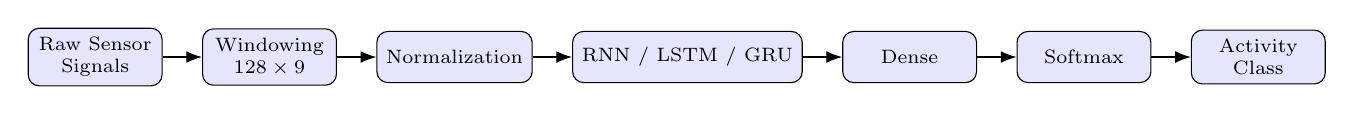
\begin{tikzpicture}[node distance=5mm]
\node[layer](a){Raw Sensor\\Signals};
\node[layer,right=of a](b){Windowing\\$128\times9$};
\node[layer,right=of b](c){Normalization};
\node[layer,right=of c](d){RNN / LSTM / GRU};
\node[layer,right=of d](e){Dense};
\node[layer,right=of e](f){Softmax};
\node[layer,right=of f](g){Activity\\Class};

\foreach \x/\y in {a/b,b/c,c/d,d/e,e/f,f/g}
\draw[arrow](\x)--(\y);
\end{tikzpicture}
\end{center}

The three recurrent models must use the same input, output layer, optimizer,
batch size and evaluation protocol.

%%%%%%%%%%%%%%%%%%%%%%%%%%%%%%%%%%%%%%%%%%%%%%%%%%%%%%%%%%%%
\section*{5. Preprocessing}

Perform the following preprocessing steps:

\begin{enumerate}
\item Load the raw inertial signals.
\item Arrange every observation window as $128\times9$.
\item Assign one activity label to each window.
\item Encode the six activity labels.
\item Normalize the input using statistics calculated from the training data.
\item Create training, validation and test sets.
\item Verify the class distribution.
\end{enumerate}

\textbf{Suggested split:}

\[
70\% \text{ training},\qquad
15\% \text{ validation},\qquad
15\% \text{ testing}.
\]

The test data must not be used during model selection or hyperparameter tuning.

\subsection*{Expected Preprocessing Output}

\begin{verbatim}
Input tensor shape:
Training   : (2100, 128, 9)
Validation : (450, 128, 9)
Testing    : (450, 128, 9)

Number of classes: 6
Number of features per time step: 9
Sequence length: 128
\end{verbatim}

A balanced pool of 3000 windows (500 per activity) was drawn from the
training partition and then split 70/15/15 into 2100 training, 450
validation and 450 test windows, with each split remaining perfectly
balanced across all six activities.

%%%%%%%%%%%%%%%%%%%%%%%%%%%%%%%%%%%%%%%%%%%%%%%%%%%%%%%%%%%%
\section*{6. Temporal Data Visualization}

Select representative sequences from at least three different activity
classes.

\figblock{plot1_sensor_signal_vs_time.png}{0.85}{Sensor signal vs. time for Body Acc X, Body Gyro X and Total Acc X, shown for WALKING, SITTING and LAYING.}

Dynamic activities show heavy oscillations across the 128 time steps, while the static activities show an almost flat trend with minor noise. SITTING and STANDING look most similar since both are stationary postures with low fluctuations, and WALKING stands apart with a strong fluctuation from the gait cycle. Activity recognition depends on this rhythm and on how signals evolve, not on any single reading. Hence, shuffling the time steps would destroy the pattern which the recurrent models depend on.

%%%%%%%%%%%%%%%%%%%%%%%%%%%%%%%%%%%%%%%%%%%%%%%%%%%%%%%%%%%%
\section*{7. Vanilla RNN Architecture}

A Vanilla RNN maintains a hidden state that is updated at every time step:

\[
h_t=\tanh(W_xx_t+W_hh_{t-1}+b_h).
\]

The output can be written as

\[
y_t=g(W_yh_t+b_y).
\]

For sequence classification, the final hidden representation can be passed
to a classifier.

\begin{center}
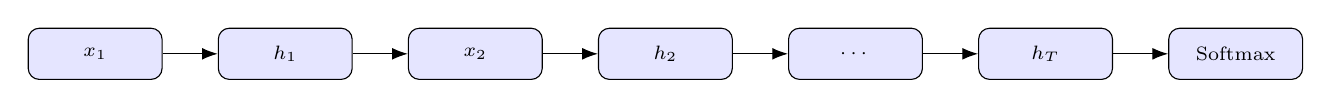
\begin{tikzpicture}[node distance=7mm]
\node[layer](x1){$x_1$};
\node[layer,right=of x1](h1){$h_1$};
\node[layer,right=of h1](x2){$x_2$};
\node[layer,right=of x2](h2){$h_2$};
\node[layer,right=of h2](x3){$\cdots$};
\node[layer,right=of x3](h3){$h_T$};
\node[layer,right=of h3](y){Softmax};

\draw[arrow](x1)--(h1);
\draw[arrow](h1)--(x2);
\draw[arrow](x2)--(h2);
\draw[arrow](h2)--(x3);
\draw[arrow](x3)--(h3);
\draw[arrow](h3)--(y);
\end{tikzpicture}
\end{center}

The diagram represents the unrolled view of an RNN. The same recurrent weights
are reused across time steps.

%%%%%%%%%%%%%%%%%%%%%%%%%%%%%%%%%%%%%%%%%%%%%%%%%%%%%%%%%%%%
\section*{8. Backpropagation Through Time}

When an RNN is unrolled, the loss depends on the sequence of hidden states.
Backpropagation Through Time (BPTT) propagates the error backward through
the recurrent steps.

\begin{center}
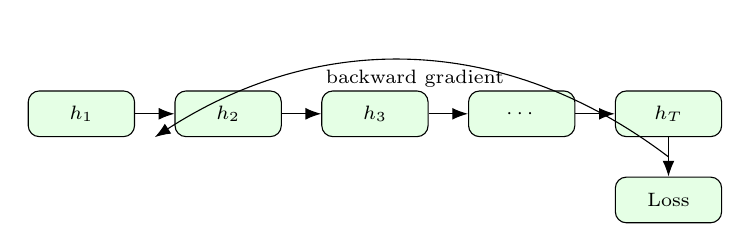
\begin{tikzpicture}[node distance=5mm]
\node[smalllayer](a){$h_1$};
\node[smalllayer,right=of a](b){$h_2$};
\node[smalllayer,right=of b](c){$h_3$};
\node[smalllayer,right=of c](d){$\cdots$};
\node[smalllayer,right=of d](e){$h_T$};
\node[smalllayer,below=of e](l){Loss};

\draw[arrow](a)--(b);
\draw[arrow](b)--(c);
\draw[arrow](c)--(d);
\draw[arrow](d)--(e);
\draw[arrow](e)--(l);

\draw[arrow]($(e.south)!0.5!(l.north)$) to[bend right=35]
node[below,font=\scriptsize]{backward gradient} ($(a.south)!0.5!(b.south)$);
\end{tikzpicture}
\end{center}

Students should explain that repeated multiplication of derivatives through
many time steps can cause gradients to become extremely small or extremely
large.

\subsection*{Challenges}

\begin{itemize}
\item Vanishing gradients
\item Exploding gradients
\item Difficulty learning long-term dependencies
\item Sequential computation and limited parallelism
\end{itemize}

The vanishing-gradient problem can be conceptually represented as

\[
\left|\frac{\partial h_t}{\partial h_{t-k}}\right|\rightarrow0
\]

while exploding gradients correspond to very large gradient magnitudes.

\subsection*{Numerical Exercise}

Consider

\[
x_1=0.5,\qquad x_2=0.7,\qquad x_3=0.2,
\]

\[
h_0=0,\qquad W_x=0.5,\qquad W_h=0.8,\qquad b=0.1.
\]

Using

\[
h_t=\tanh(W_xx_t+W_hh_{t-1}+b),
\]

the manually calculated values were:

\[
h_1 = 0.336376,\qquad h_2 = 0.616352,\qquad h_3 = 0.599958.
\]

These values were verified against a TensorFlow \texttt{SimpleRNNCell}
initialized with the same weights, which produced $h_1 = 0.336376$,
$h_2 = 0.616352$ and $h_3 = 0.599958$ -- matching the hand calculation to
within $3\times10^{-8}$, confirming the manual derivation is correct.

%%%%%%%%%%%%%%%%%%%%%%%%%%%%%%%%%%%%%%%%%%%%%%%%%%%%%%%%%%%%
\section*{9. RNN Implementation}

Use a small recurrent architecture:

\begin{center}
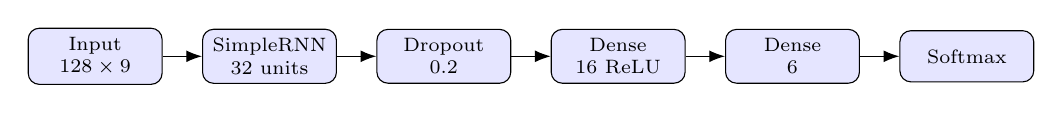
\begin{tikzpicture}[node distance=5mm]
\node[layer](a){Input\\$128\times9$};
\node[layer,right=of a](b){SimpleRNN\\32 units};
\node[layer,right=of b](c){Dropout\\0.2};
\node[layer,right=of c](d){Dense\\16 ReLU};
\node[layer,right=of d](e){Dense\\6};
\node[layer,right=of e](f){Softmax};

\foreach \x/\y in {a/b,b/c,c/d,d/e,e/f}
\draw[arrow](\x)--(\y);
\end{tikzpicture}
\end{center}

\textbf{Training configuration used:}

\begin{center}
\begin{tabular}{|l|l|}
\hline
Parameter & Value\\
\hline
Recurrent units & 32\\
Dropout & 0.2\\
Optimizer & Adam\\
Learning rate & $10^{-3}$\\
Batch size & 32\\
Epochs & 30\\
Loss & Sparse categorical cross-entropy\\
\hline
\end{tabular}
\end{center}

%%%%%%%%%%%%%%%%%%%%%%%%%%%%%%%%%%%%%%%%%%%%%%%%%%%%%%%%%%%%
\section*{10. LSTM Architecture}

LSTM introduces a memory cell and gates to control information flow.

The forget gate is

\[
f_t=\sigma(W_f[h_{t-1},x_t]+b_f),
\]

the input gate is

\[
i_t=\sigma(W_i[h_{t-1},x_t]+b_i),
\]

and the output gate is

\[
o_t=\sigma(W_o[h_{t-1},x_t]+b_o).
\]

The candidate cell state is

\[
\tilde{C}_t=
\tanh(W_C[h_{t-1},x_t]+b_C),
\]

and the cell state is

\[
C_t=f_tC_{t-1}+i_t\tilde{C}_t.
\]

The hidden state is

\[
h_t=o_t\tanh(C_t).
\]

\begin{center}
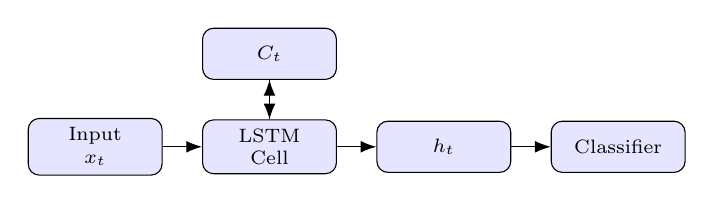
\begin{tikzpicture}[node distance=5mm]
\node[layer](a){Input\\$x_t$};
\node[layer,right=of a](b){LSTM\\Cell};
\node[layer,right=of b](c){$h_t$};
\node[layer,above=of b](d){$C_t$};
\node[layer,right=of c](e){Classifier};

\draw[arrow](a)--(b);
\draw[arrow](b)--(c);
\draw[arrow](b)--(d);
\draw[arrow](c)--(e);
\draw[arrow](d)--(b);
\end{tikzpicture}
\end{center}

\textbf{Required inference:} Explain how the cell state and gates help the
network retain or discard information over long sequences.

%%%%%%%%%%%%%%%%%%%%%%%%%%%%%%%%%%%%%%%%%%%%%%%%%%%%%%%%%%%%
\section*{11. GRU Architecture}

GRU uses two principal gates:

\[
z_t=\sigma(W_z[h_{t-1},x_t]+b_z)
\]

and

\[
r_t=\sigma(W_r[h_{t-1},x_t]+b_r).
\]

The candidate hidden state is

\[
\tilde{h}_t=
\tanh(W_h[r_t\odot h_{t-1},x_t]+b_h).
\]

The hidden state is updated using

\[
h_t=(1-z_t)h_{t-1}+z_t\tilde{h}_t.
\]

\begin{center}
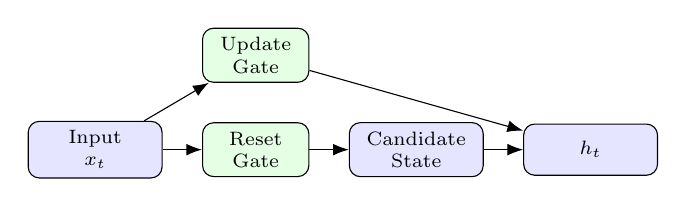
\begin{tikzpicture}[node distance=5mm]
\node[layer](a){Input\\$x_t$};
\node[smalllayer,right=of a](b){Reset\\Gate};
\node[smalllayer,above=of b](c){Update\\Gate};
\node[layer,right=of b](d){Candidate\\State};
\node[layer,right=of d](e){$h_t$};

\draw[arrow](a)--(b);
\draw[arrow](a)--(c);
\draw[arrow](b)--(d);
\draw[arrow](c)--(e);
\draw[arrow](d)--(e);
\end{tikzpicture}
\end{center}

Students should compare the number of gates and state representations in
RNN, LSTM and GRU.

%%%%%%%%%%%%%%%%%%%%%%%%%%%%%%%%%%%%%%%%%%%%%%%%%%%%%%%%%%%%
\section*{12. LSTM and GRU Implementation}

Implement the same classifier used for the RNN, replacing only the recurrent
layer.

\begin{center}
\begin{tabular}{|l|c|c|c|}
\hline
Model & Recurrent Layer & Units & Output Classes\\
\hline
RNN & SimpleRNN & 32 & 6\\
LSTM & LSTM & 32 & 6\\
GRU & GRU & 32 & 6\\
\hline
\end{tabular}
\end{center}

All other experimental conditions remained unchanged.


\figblock{plot2_loss_curves.png}{1.0}{Training and validation loss curves for RNN, LSTM and GRU over 30 epochs.}


\figblock{plot3_accuracy_curves.png}{1.0}{Training and validation accuracy curves for RNN, LSTM and GRU over 30 epochs.}

RNN's loss and accuracy curves flatten at around epoch 20 with training accuracy near 80\% and a validation curve which follows closely. This shows slow and limited convergence without much overfitting. LSTM and GRU both converge much faster than RNN, converging at around epoch 10, and also have lower validation loss and higher validation accuracy. Their validation curves stay close to the training curves throughout, which means there is no overfitting and there is proper generalization. RNN struggles to retain information over 128 time steps, while the gating mechanisms in LSTM and GRU let them learn the same task faster and more completely on this same balanced split.

%%%%%%%%%%%%%%%%%%%%%%%%%%%%%%%%%%%%%%%%%%%%%%%%%%%%%%%%%%%%
\section*{13. Performance Evaluation}

Each model was evaluated on the independent test set.


\begin{center}
\begin{tabular}{|l|c|c|c|}
\hline
Metric & RNN & LSTM & GRU\\
\hline
Accuracy (\%) & 82.00 & 95.56 & 94.67\\
Macro Precision (\%) & 81.88 & 95.65 & 95.30\\
Macro Recall (\%) & 82.00 & 95.56 & 94.67\\
Macro F1 (\%) & 81.88 & 95.55 & 94.60\\
Parameters & 1{,}974 & 6{,}006 & 4{,}758\\
Training Time (s) & 27.45 & 23.49 & 20.88\\
\hline
\end{tabular}
\end{center}

%%%%%%%%%%%%%%%%%%%%%%%%%%%%%%%%%%%%%%%%%%%%%%%%%%%%%%%%%%%%
\section*{14. Confusion Matrix Analysis}

\figblock{plot4_confusion_matrices.png}{1.0}{Confusion matrices for RNN, LSTM and GRU on the held-out test set.}

Across all three models, LAYING is recognized almost perfectly since its sensor signature is the most distinct from the other five activities, while the most consistent confusion is between SITTING and STANDING, both static postures with very similar sensor traces. RNN shows some error in distinguishing between WALKING\_UPSTAIRS and WALKING\_DOWNSTAIRS, which LSTM and GRU handle better. This shows that plain RNN has a weaker ability to recognize and remember fine temporal cues. All 3 models show similar errors, but RNN shows slightly worser distinguision.

%%%%%%%%%%%%%%%%%%%%%%%%%%%%%%%%%%%%%%%%%%%%%%%%%%%%%%%%%%%%
\section*{15. RNN vs. LSTM vs. GRU Comparison}

\begin{center}
\begin{tabular}{|l|c|c|c|}
\hline
Property & RNN & LSTM & GRU\\
\hline
Hidden state & Yes & Yes & Yes\\
Cell state & No & Yes & No\\
Forget gate & No & Yes & No\\
Input gate & No & Yes & No\\
Output gate & No & Yes & No\\
Update gate & No & No & Yes\\
Reset gate & No & No & Yes\\
Parameters & 1{,}974 & 6{,}006 & 4{,}758\\
Training time & 27.45s & 23.49s & 20.88s\\
Test F1-score & 81.88 & 95.55 & 94.60\\
\hline
\end{tabular}
\end{center}

\figblock{plot5_model_comparison.png}{0.75}{Bar plot comparing test accuracy, macro F1-score, and normalized parameter count and training time for RNN, LSTM and GRU.}

LSTM performs best despite having the most parameters and taking roughly same training time as GRU. GRU also performs well, with only slightly lagging behind LSTM, and trains the fastest. Regular RNN takes the highest training time even though it has the least parameters, and also gave the worst results. GRU trains fastest and uses a medium amount of parameters, showing a good trade off as it performs only slightly poor than LSTM. LSTM gives better results with slightly more parameters and training time.  

%%%%%%%%%%%%%%%%%%%%%%%%%%%%%%%%%%%%%%%%%%%%%%%%%%%%%%%%%%%%
\section*{16. Effect of Sequence Length}

To understand temporal dependency, the experiment was repeated using selected
sequence lengths:

\[
T\in\{32,64,128\}.
\]

\begin{center}
\begin{tabular}{|c|c|c|c|}
\hline
Sequence Length & RNN F1 & LSTM F1 & GRU F1\\
\hline
32 & 80.34 & 94.42 & 92.10\\
64 & 85.90 & 95.33 & 92.99\\
128 & 80.22 & 93.08 & 95.31\\
\hline
\end{tabular}
\end{center}

\figblock{plot6_sequence_length_vs_f1.png}{0.75}{Test macro F1-score against sequence length for RNN, LSTM and GRU.}

GRU's F1-score increases steadily with sequence length, and performs best with 128 steps, showing that it performs best with more temporal context. LSTM performs well at all 3 lengths, but best at 64 and slightly dipping at 128. RNN is less stable, peaking at 64 and performing poor at 32 and 128, showing that it loses information over longer unrolled sequences. This shows that LSTM and GRU can handle data of longer length, while regular RNN fails as length increases due to vanishing gradients problem.

%%%%%%%%%%%%%%%%%%%%%%%%%%%%%%%%%%%%%%%%%%%%%%%%%%%%%%%%%%%%
\section*{17. Video Understanding Using CNN and RNN}

This part demonstrates the application:

\[
\boxed{\text{Video Understanding using CNN + RNN}}
\]

A video is a sequence of image frames. CNNs are used to extract spatial
features from individual frames, while RNN/LSTM/GRU models the temporal
relationship among those features.

The complete pipeline is:

\begin{center}
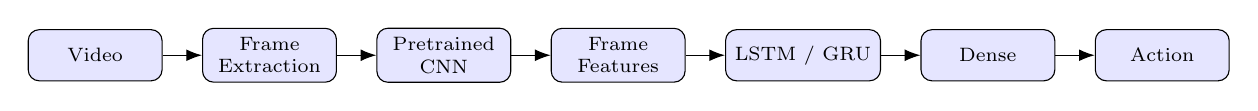
\begin{tikzpicture}[node distance=5mm]
\node[layer](a){Video};
\node[layer,right=of a](b){Frame\\Extraction};
\node[layer,right=of b](c){Pretrained\\CNN};
\node[layer,right=of c](d){Frame\\Features};
\node[layer,right=of d](e){LSTM / GRU};
\node[layer,right=of e](f){Dense};
\node[layer,right=of f](g){Action};

\foreach \x/\y in {a/b,b/c,c/d,d/e,e/f,f/g}
\draw[arrow](\x)--(\y);
\end{tikzpicture}
\end{center}

\subsection*{Dataset Used}

A subset of the UCF101 action-recognition dataset
(\url{https://www.crcv.ucf.edu/data/UCF101.php}) was used, restricted to
five action classes with 40 videos sampled per class (200 videos total, of
which 188 produced usable frame sequences):

\begin{itemize}
\item Biking
\item CricketShot
\item PushUps
\item TableTennisShot
\item TennisSwing
\end{itemize}

The objective is to understand the CNN--recurrent pipeline rather than to
train a state-of-the-art video recognition system.

%%%%%%%%%%%%%%%%%%%%%%%%%%%%%%%%%%%%%%%%%%%%%%%%%%%%%%%%%%%%
\section*{18. Expected Video Input and Output}

10 frames were sampled uniformly from each video, each resized to
$224\times224\times3$.

MobileNetV2, used only as a feature extractor, produced a feature vector of
dimension $D=1280$, so the recurrent network received

\[
X\in\mathbb{R}^{10\times1280}
\]

per video, and for a batch of $B$ videos, $X\in\mathbb{R}^{B\times10\times1280}$.

Sample predictions obtained directly from the trained CNN--LSTM model on
the full test set (confidence values are model outputs, not manually
entered):

\begin{verbatim}
[ 1] Predicted: TableTennisShot | Actual: TableTennisShot | Confidence: 0.99
[ 5] Predicted: TennisSwing     | Actual: TennisSwing     | Confidence: 0.99
[ 6] Predicted: PushUps         | Actual: PushUps         | Confidence: 0.98
[ 7] Predicted: TableTennisShot | Actual: TableTennisShot | Confidence: 1.00
[ 8] Predicted: CricketShot     | Actual: CricketShot     | Confidence: 0.98
[ 9] Predicted: CricketShot     | Actual: CricketShot     | Confidence: 0.97
[10] Predicted: Biking          | Actual: Biking          | Confidence: 0.84
[11] Predicted: TableTennisShot | Actual: TableTennisShot | Confidence: 0.99
[12] Predicted: CricketShot     | Actual: CricketShot     | Confidence: 0.90
[13] Predicted: PushUps         | Actual: CricketShot     | Confidence: 0.94
[14] Predicted: CricketShot     | Actual: CricketShot     | Confidence: 0.99
[15] Predicted: TableTennisShot | Actual: TableTennisShot | Confidence: 1.00
[16] Predicted: TennisSwing     | Actual: Biking          | Confidence: 0.66
[17] Predicted: TennisSwing     | Actual: TennisSwing     | Confidence: 0.99
[18] Predicted: PushUps         | Actual: PushUps         | Confidence: 1.00
[19] Predicted: PushUps         | Actual: PushUps         | Confidence: 1.00
[20] Predicted: TennisSwing     | Actual: TennisSwing     | Confidence: 0.99
[21] Predicted: TableTennisShot | Actual: TableTennisShot | Confidence: 0.97
[22] Predicted: CricketShot     | Actual: TennisSwing     | Confidence: 0.94
[23] Predicted: TableTennisShot | Actual: TableTennisShot | Confidence: 1.00
[24] Predicted: TennisSwing     | Actual: TennisSwing     | Confidence: 1.00
[25] Predicted: CricketShot     | Actual: CricketShot     | Confidence: 0.99
[26] Predicted: PushUps         | Actual: PushUps         | Confidence: 1.00
[27] Predicted: PushUps         | Actual: PushUps         | Confidence: 0.99
[28] Predicted: PushUps         | Actual: PushUps         | Confidence: 1.00
[29] Predicted: Biking          | Actual: Biking          | Confidence: 0.99
\end{verbatim}

%%%%%%%%%%%%%%%%%%%%%%%%%%%%%%%%%%%%%%%%%%%%%%%%%%%%%%%%%%%%
\section*{19. CNN Feature Extraction}

A pretrained MobileNetV2 was used with the classification head removed.

\begin{center}
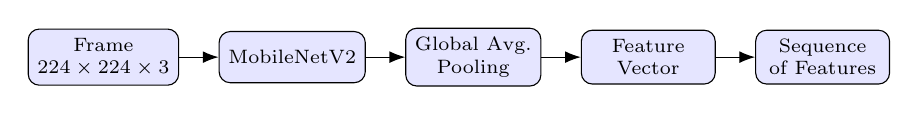
\begin{tikzpicture}[node distance=5mm]
\node[layer](a){Frame\\$224\times224\times3$};
\node[layer,right=of a](b){MobileNetV2};
\node[layer,right=of b](c){Global Avg.\\Pooling};
\node[layer,right=of c](d){Feature\\Vector};
\node[layer,right=of d](e){Sequence\\of Features};

\foreach \x/\y in {a/b,b/c,c/d,d/e}
\draw[arrow](\x)--(\y);
\end{tikzpicture}
\end{center}

The CNN was not trained from scratch; it was frozen and used purely for
feature extraction before the recurrent classifier was trained.

The CNN feature dimension obtained was $D=1280$, and the resulting tensor
shape supplied to the recurrent network was $(188, 10, 1280)$, i.e. 188
usable videos, 10 sampled frames each, and a 1280-dimensional MobileNetV2
feature vector per frame.

%%%%%%%%%%%%%%%%%%%%%%%%%%%%%%%%%%%%%%%%%%%%%%%%%%%%%%%%%%%%
\section*{20. CNN--LSTM / CNN--GRU Model}

The architecture used:

\begin{center}
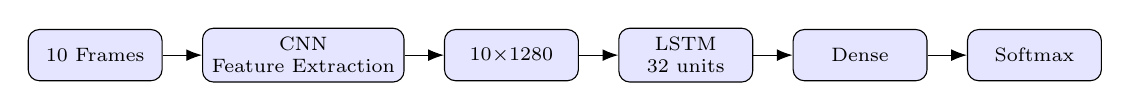
\begin{tikzpicture}[node distance=5mm]
\node[layer](a){10 Frames};
\node[layer,right=of a](b){CNN\\Feature Extraction};
\node[layer,right=of b](c){10$\times$1280};
\node[layer,right=of c](d){LSTM\\32 units};
\node[layer,right=of d](e){Dense};
\node[layer,right=of e](f){Softmax};

\foreach \x/\y in {a/b,b/c,c/d,d/e,e/f}
\draw[arrow](\x)--(\y);
\end{tikzpicture}
\end{center}

\figblock{plot7_video_sample_frames.png}{0.9}{Ten uniformly sampled frames from a representative video.}

CNN extracts spatial appearance cues from each individual frame, like body pose, equipment (bat, racquet, etc) and surrounding scene, Recurrent network then learns how this sequence of frame descriptions changes across the 10 sampled frames, capturing the motion pattern, like pedalling, taking pushups, swinging bat or arm, etc, and distinguishes them.\\\\


\figblock{plot8_video_training_curves.png}{1.0}{Training and validation loss and accuracy for the CNN--LSTM video classifier over 30 epochs.}

Both training and validation accuracy reach 100\% within the first few epochs and the loss drops close to zero, which is caused by the very small dataset size (131 training videos across 5 classes) relative to the LSTM's capacity. This is a case where the model easily memorizing a small, visually distinct set of training videos, and it is because should be read as a limitation of the available data volume rather than evidence of a strong general video classifier.\\


\figblock{plot9_video_confusion_matrix.png}{0.6}{Confusion matrix for the CNN--LSTM video classifier on the test set.}

Confusion matrix's diagonals show that most classes are recognized correctly. Errors are concentrated around TennisSwing, CricketShot and Biking, possibly since all involve arm motion captured from similar camera angles in this subset. This shows that the minor confusion is caused by patterns which look visually similar over just 10 sampled frames.

%%%%%%%%%%%%%%%%%%%%%%%%%%%%%%%%%%%%%%%%%%%%%%%%%%%%%%%%%%%%
\section*{21. Sequence-to-Sequence Learning}

Sequence-to-sequence learning maps one sequence to another.

For a simple laboratory task, a synthetic reversal dataset was constructed:

\[
[1,4,7,2]\rightarrow[2,7,4,1].
\]

5000 short sequences of length 4 were generated using integers from 1--9,
split 70/15/15 into 3500 training, 750 validation and 750 test examples.

\begin{center}
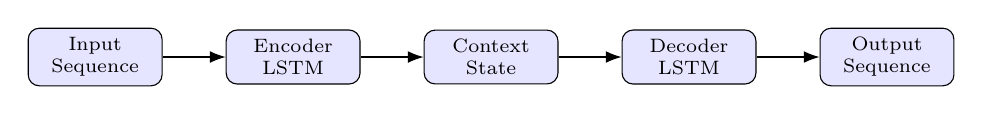
\begin{tikzpicture}[node distance=8mm]
\node[layer](a){Input\\Sequence};
\node[layer,right=of a](b){Encoder\\LSTM};
\node[layer,right=of b](c){Context\\State};
\node[layer,right=of c](d){Decoder\\LSTM};
\node[layer,right=of d](e){Output\\Sequence};

\foreach \x/\y in {a/b,b/c,c/d,d/e}
\draw[arrow](\x)--(\y);
\end{tikzpicture}
\end{center}

The encoder converts the input sequence into a learned representation.
The decoder generates the output sequence one element at a time.

%%%%%%%%%%%%%%%%%%%%%%%%%%%%%%%%%%%%%%%%%%%%%%%%%%%%%%%%%%%%
\section*{22. Expected Sequence-to-Sequence Input and Output}

Example input: $[3,8,1,5]$, expected output: $[5,1,8,3]$.

Five test examples obtained from the trained encoder--decoder model:

\begin{center}
\begin{tabular}{|c|c|c|}
\hline
Sample & Input Sequence & Predicted Output\\
\hline
1 & [4, 9, 8, 6] & [6, 8, 9, 4]\\
2 & [4, 3, 5, 9] & [9, 5, 3, 4]\\
3 & [9, 3, 8, 1] & [1, 8, 3, 9]\\
4 & [9, 8, 6, 3] & [3, 6, 8, 9]\\
5 & [3, 7, 3, 9] & [9, 3, 7, 3]\\
\hline
\end{tabular}
\end{center}

%%%%%%%%%%%%%%%%%%%%%%%%%%%%%%%%%%%%%%%%%%%%%%%%%%%%%%%%%%%%
\section*{23. Sequence-to-Sequence Evaluation}

\begin{itemize}
\item Token Accuracy: 100.00\%
\item Sequence Accuracy: 100.00\%
\item Final Training Loss: 0.0030
\item Final Validation Loss: 0.0037
\end{itemize}

Token accuracy is

\[
\text{Token Accuracy}
=
\frac{\text{Correctly predicted tokens}}
{\text{Total tokens}}.
\]

Sequence accuracy is

\[
\text{Sequence Accuracy}
=
\frac{\text{Completely correct sequences}}
{\text{Total sequences}}.
\]

Sequence-level accuracy can fall well below token accuracy because a
sequence only counts as correct when every single token in it is correct,
so even a model that gets 95\% of individual tokens right can have a much
lower fraction of fully correct sequences once the errors are spread across
different examples. In this experiment both metrics reached 100\% because
reversing a length-4 sequence is a simple, fully learnable transformation
for an LSTM encoder--decoder given 5000 training examples, so the two
metrics happened to coincide rather than diverge.

%%%%%%%%%%%%%%%%%%%%%%%%%%%%%%%%%%%%%%%%%%%%%%%%%%%%%%%%%%%%
\section*{24. Consolidated Results}

\begin{center}
\begin{tabular}{|l|c|c|c|c|c|}
\hline
Model & Accuracy (\%) & Precision (\%) & Recall (\%) & F1 (\%) & Parameters\\
\hline
RNN & 82.00 & 81.88 & 82.00 & 81.88 & 1{,}974\\
LSTM & 95.56 & 95.65 & 95.56 & 95.55 & 6{,}006\\
GRU & 94.67 & 95.30 & 94.67 & 94.60 & 4{,}758\\
CNN--LSTM & 89.66 & 89.81 & 89.33 & 89.31 & 168{,}229\\
\hline
\end{tabular}
\end{center}

\textbf{Sequence-to-sequence task results:}

\begin{center}
\begin{tabular}{|l|c|}
\hline
Metric & Value\\
\hline
Token Accuracy (\%) & 100.00\\
Sequence Accuracy (\%) & 100.00\\
Training Loss & 0.0030\\
Validation Loss & 0.0037\\
\hline
\end{tabular}
\end{center}

%%%%%%%%%%%%%%%%%%%%%%%%%%%%%%%%%%%%%%%%%%%%%%%%%%%%%%%%%%%%

\section*{25. Source Code}

The repository contains a single Kaggle notebook implementing the complete pipeline described in this report, from HAR preprocessing through RNN/LSTM/GRU training, the CNN--LSTM video model, and the sequence-to-sequence task, along with all seven additional exercises and every generated figure:\\

    \hspace{25mm}  \url{https://github.com/Ashwin271206/dl-lab/tree/main/Lab%206}\\

The repository contains a single Kaggle notebook covering all tasks experimented in this report, along with the generated figures and outputs.

%%%%%%%%%%%%%%%%%%%%%%%%%%%%%%%%%%%%%%%%%%%%%%%%%%%%%%%%%%%%

\section*{26. Discussion Questions}

\begin{enumerate}
\item \textbf{What is a recurrent neural network?} \\A neural network with a feedback loop in its hidden layer, so the output at each time step depends on both the current input and the network's own previous hidden state.
\item \textbf{What information is represented by the hidden state?} \\A compressed summary of everything the network has seen in the sequence so far, updated at every time step.
\item \textbf{Why is sequence order important?} \\Reordering the inputs changes the hidden state trajectory and therefore the meaning of the sequence; temporal or positional dependencies would be lost if order were ignored.
\item \textbf{Explain the difference between a feed-forward network and an RNN.} \\A feed-forward network maps each input independently with no memory between samples, while an RNN carries a hidden state across time steps, letting past inputs influence the processing of later ones.
\item \textbf{Explain Backpropagation Through Time.} \\BPTT unrolls the RNN across all time steps and applies standard backpropagation on this unrolled graph, accumulating gradients for the shared weights across every time step the loss depends on.
\item \textbf{Why can gradients vanish during BPTT?} \\Because the gradient at an early time step is a product of many Jacobians (one per time step); if these have magnitude less than 1, the product shrinks toward zero over long sequences.
\item \textbf{Why can gradients explode during BPTT?} \\By the same repeated-multiplication mechanism, if the per-step Jacobians have magnitude greater than 1, the product can grow extremely large instead of shrinking.
\item \textbf{What are long-term dependencies?} \\Relationships between elements that are far apart in a sequence, where correctly predicting a later element requires remembering information from much earlier time steps.
\item \textbf{What is the role of the LSTM cell state?} \\It acts as a relatively unobstructed memory channel that can carry information across many time steps with only gated, additive updates, avoiding the repeated multiplicative squashing that causes vanishing gradients.
\item \textbf{What are the forget, input and output gates in LSTM?} \\The forget gate decides what to discard from the cell state, the input gate decides what new information to write into it, and the output gate decides what part of the cell state to expose as the hidden state.
\item \textbf{What are the reset and update gates in GRU?} \\The reset gate controls how much of the previous hidden state is used when computing the candidate state, and the update gate controls the blend between the previous hidden state and the new candidate state.
\item \textbf{Compare LSTM and GRU.} \\LSTM has three gates and a separate cell state, giving it more expressive control but more parameters; GRU merges the cell and hidden state and uses only two gates, making it lighter and often faster to train with comparable accuracy.
\item \textbf{Why does GRU generally use a simpler gating mechanism than LSTM?} \\GRU was designed to achieve similar gating benefits with fewer parameters by combining the forget and input gates into a single update gate and dropping the separate cell state.
\item \textbf{Why should RNN, LSTM and GRU be compared using the same experimental settings?} \\So that any difference in performance can be attributed to the recurrent architecture itself rather than to differences in data, preprocessing, optimizer or training budget.
\item \textbf{What does the confusion matrix reveal that accuracy alone does not?} \\It shows which specific classes are being confused with which others, exposing systematic error patterns (like SITTING vs STANDING here) that a single accuracy number would hide.
\item \textbf{Why should macro F1-score be reported for multi-class classification?} \\Because it averages the F1-score across classes without weighting by class frequency, so it does not let performance on a majority class mask poor performance on a minority class.
\item \textbf{What is the significance of sequence length?} \\It determines how much temporal context the model has access to; too short a sequence may omit information needed for classification, while too long a sequence increases the risk of vanishing gradients for simpler architectures.
\item \textbf{Why can a CNN be used as a feature extractor for video?} \\Because a CNN pretrained on large image datasets already learns general-purpose spatial features (edges, textures, object parts) that transfer well to describing the content of individual video frames.
\item \textbf{What type of information is extracted by the CNN?} \\Spatial, appearance-based information from each frame in isolation, such as objects, poses and scene context.
\item \textbf{What type of information is learned by the recurrent network?} \\Temporal information, i.e. how the CNN's per-frame features change and evolve across the sampled frames.
\item \textbf{Why are CNN features arranged as a sequence before being given to LSTM/GRU?} \\Because the recurrent layer expects a sequence of feature vectors, one per time step, so that it can model how the frame-level representations evolve over the video's duration.
\item \textbf{Explain the encoder and decoder in sequence-to-sequence learning.} \\The encoder reads the entire input sequence and compresses it into a fixed context representation; the decoder then generates the output sequence one token at a time, conditioned on that context and on the tokens it has generated so far.
\item \textbf{What is teacher forcing?} \\A training technique where the decoder is fed the ground-truth previous token as input at each step, rather than its own prediction, which speeds up and stabilizes training.
\item \textbf{Differentiate token accuracy and sequence accuracy.} \\Token accuracy measures the fraction of individual output positions predicted correctly, while sequence accuracy measures the fraction of entire output sequences that are completely correct, and is therefore always less than or equal to token accuracy.
\item \textbf{Why must the test set remain untouched during model selection?} \\Using the test set to guide model or hyperparameter choices would let information from it leak into the training process, giving an overly optimistic and unreliable estimate of how the model performs on genuinely unseen data.
\end{enumerate}

%%%%%%%%%%%%%%%%%%%%%%%%%%%%%%%%%%%%%%%%%%%%%%%%%%%%%%%%%%%%
\section*{27. Additional Exercises}

\subsection*{27.1 Effect of Recurrent Units (16 vs 32 vs 64)}

Each of RNN, LSTM and GRU was retrained with 16, 32 and 64 recurrent units, keeping all other settings identical.

\begin{center}
\begin{tabular}{|l|c|c|c|c|c|}
\hline
Model & Units & Accuracy (\%) & F1 (\%) & Parameters & Training Time (s)\\
\hline
RNN & 16 & 74.00 & 73.85 & 790 & 26.87\\
LSTM & 16 & 94.89 & 94.87 & 2{,}038 & 21.44\\
GRU & 16 & 93.56 & 93.51 & 1{,}670 & 21.22\\
RNN & 32 & 81.33 & 81.37 & 1{,}974 & 26.60\\
LSTM & 32 & 96.00 & 96.00 & 6{,}006 & 21.67\\
GRU & 32 & 94.67 & 94.64 & 4{,}758 & 21.14\\
RNN & 64 & 79.11 & 78.87 & 5{,}878 & 27.50\\
LSTM & 64 & 92.67 & 92.50 & 20{,}086 & 21.60\\
GRU & 64 & 96.22 & 96.22 & 15{,}542 & 21.34\\
\hline
\end{tabular}
\end{center}

Increasing the unit count grows the RNN's parameter count steeply but does not translate into better accuracy, and its best result is actually at 32 units, suggesting it is not data- or context-limited but architecturally limited. LSTM peaks at 32 units and slightly drops at 64, hinting at mild overfitting with the extra capacity on this small dataset, while GRU keeps improving up to 64 units and reaches its best overall F1-score there, showing it makes the most efficient use of added capacity among the three.

\subsection*{27.2 GRU vs LSTM Using the Same Number of Recurrent Units}

\begin{center}
\begin{tabular}{|l|c|c|c|c|}
\hline
Model & Accuracy (\%) & F1 (\%) & Parameters & Training Time (s)\\
\hline
LSTM & 96.00 & 96.00 & 6{,}006 & 21.67\\
GRU & 94.67 & 94.64 & 4{,}758 & 21.14\\
\hline
\end{tabular}
\end{center}

At an identical 32 units, LSTM edges out GRU by about 1.3 percentage points in both accuracy and F1-score, at the cost of roughly 26\% more parameters, while the two take almost the same time to train. This is a small but consistent gap in favour of LSTM's extra gate on this HAR task, though GRU remains competitive given its lighter parameter footprint.

\subsection*{27.3 Effect of Adding a Second Recurrent Layer}

\begin{center}
\begin{tabular}{|l|c|c|c|c|}
\hline
Model & Accuracy (\%) & F1 (\%) & Parameters & Training Time (s)\\
\hline
RNN (2-layer) & 90.22 & 90.22 & 4{,}054 & 43.96\\
LSTM (2-layer) & 96.22 & 96.22 & 14{,}326 & 31.18\\
GRU (2-layer) & 95.33 & 95.33 & 11{,}094 & 30.56\\
\hline
\end{tabular}
\end{center}

Stacking a second recurrent layer helps every architecture, and the RNN benefits the most dramatically, jumping from 81.33\% to 90.22\% accuracy, since the extra layer partly compensates for its weaker single-layer temporal modeling. LSTM and GRU also improve modestly, but at roughly double the training time and 2--3$\times$ the parameters of their single-layer counterparts, so the accuracy gain has to be weighed against a real increase in computational cost.

\subsection*{27.4 Bidirectional LSTM vs. Unidirectional LSTM}

\begin{center}
\begin{tabular}{|l|c|c|c|c|}
\hline
Model & Accuracy (\%) & F1 (\%) & Parameters & Training Time (s)\\
\hline
LSTM (unidirectional) & 95.56 & 95.55 & 6{,}006 & 23.49\\
BiLSTM & 91.33 & 90.82 & 11{,}894 & 30.12\\
\hline
\end{tabular}
\end{center}

Contrary to the usual expectation that bidirectionality helps, the BiLSTM here performs worse than the unidirectional LSTM despite roughly doubling the parameter count and training time. This is most likely because the smaller 2100-sample training set is not large enough to reliably train the extra backward-pass parameters, so the added capacity leads to a harder optimization problem rather than a benefit on this particular balanced HAR subset.

\subsection*{27.5 Sequence Length vs. Computational Cost}

\figblock{exercise5_seqlen_vs_cost.png}{0.75}{Training time against sequence length for RNN, LSTM and GRU.}

\begin{center}
\begin{tabular}{|c|c|c|c|}
\hline
Sequence Length & RNN Time (s) & LSTM Time (s) & GRU Time (s)\\
\hline
32 & 17.0 & 17.0 & 16.2\\
64 & 19.4 & 17.8 & 17.5\\
128 & 26.3 & 20.9 & 20.6\\
\hline
\end{tabular}
\end{center}

Training time grows with sequence length for all three architectures, as expected since more time steps mean more repeated recurrent computation per sample. The RNN's training time grows the fastest of the three, roughly 55\% slower at $T=128$ than at $T=32$, while LSTM and GRU scale more gently, showing that their internal gating, despite adding per-step computation, does not disproportionately increase overall training cost as sequences get longer.

\subsection*{27.6 Video Task: LSTM vs. GRU on Identical CNN Features}

\begin{center}
\begin{tabular}{|l|c|c|c|c|}
\hline
Model & Accuracy (\%) & F1 (\%) & Parameters & Training Time (s)\\
\hline
CNN--LSTM & 93.10 & 92.91 & 168{,}229 & 6.76\\
CNN--GRU & 96.55 & 96.64 & 126{,}309 & 6.69\\
\hline
\end{tabular}
\end{center}

On identical MobileNetV2 features, CNN--GRU outperforms CNN--LSTM on both accuracy and F1-score while using about 25\% fewer parameters, mirroring the pattern seen in Exercise 1 where GRU made more efficient use of a small dataset. This suggests that for this video task's limited sample size, GRU's lighter parameterization is an advantage rather than a limitation.

\subsection*{27.7 Seq2Seq With Output Sequence Length Different From Input}

The reversal task was modified so the encoder reads an input of length 4 but the decoder produces only the first 2 tokens of the reversed sequence (e.g. input $[1,3,3,5] \to$ output $[5,3]$).

\begin{itemize}
\item Input length: 4, Output length: 2
\item Final Training Loss: 0.0012
\item Final Validation Loss: 0.0012
\item Example: Input $[1, 3, 3, 5] \to$ Predicted Output $[5, 3]$
\end{itemize}

The encoder--decoder framework handles the length mismatch naturally, since the encoder's fixed-size context vector does not depend on the output length, and the decoder simply stops generating after 2 steps instead of 4. Training loss converges to an even lower value than the original equal-length task, confirming that decoding a shorter, simpler output sequence is, if anything, an easier learning problem for the same architecture.

%%%%%%%%%%%%%%%%%%%%%%%%%%%%%%%%%%%%%%%%%%%%%%%%%%%%%%%%%%%%
\section*{28. Expected Outcome}

At the end of the experiment, students should be able to demonstrate the
complete sequence-learning pipeline:

\[
\boxed{
\text{Sequential Data}
\rightarrow
\text{Preprocessing}
\rightarrow
\text{RNN/LSTM/GRU}
\rightarrow
\text{Evaluation}
}
\]

and the video-understanding pipeline:

\[
\boxed{
\text{Video}
\rightarrow
\text{Frames}
\rightarrow
\text{CNN Features}
\rightarrow
\text{LSTM/GRU}
\rightarrow
\text{Action Prediction}
}
\]

They should also understand the encoder--decoder formulation:

\[
\boxed{
\text{Input Sequence}
\rightarrow
\text{Encoder}
\rightarrow
\text{Context}
\rightarrow
\text{Decoder}
\rightarrow
\text{Output Sequence}
}
\]

The final report should demonstrate both implementation and interpretation.
Numerical performance values must be obtained from the student's own
execution and should not be assumed in advance.

%%%%%%%%%%%%%%%%%%%%%%%%%%%%%%%%%%%%%%%%%%%%%%%%%%%%%%%%%%%%
\section*{29. References}

\begin{enumerate}
\item Ian Goodfellow, Yoshua Bengio and Aaron Courville,
\emph{Deep Learning}, MIT Press, 2016.

\item Sepp Hochreiter and Jürgen Schmidhuber,
``Long Short-Term Memory,'' \emph{Neural Computation}, 1997.

\item Kyunghyun Cho et al.,
``Learning Phrase Representations using RNN Encoder--Decoder for Statistical
Machine Translation,'' EMNLP, 2014.

\item Anguita et al.,
``A Public Domain Dataset for Human Activity Recognition Using Smartphones,''
ESANN, 2013.

\item Khurram Soomro, Amir Roshan Zamir and Mubarak Shah,
``UCF101: A Dataset of 101 Human Actions Classes From Videos in the Wild,''
2012.

\item TensorFlow Documentation:
\url{https://www.tensorflow.org}

\item Keras Documentation:
\url{https://keras.io}
\end{enumerate}

\end{document}